\newpage
\section{Conclusión}
\subsection{Presentación de resultados}

A continuación presentamos los resultados de la encuesta \textbf{"Uso de tecnologías multiplataforma en el desarrollo de aplica-
ciones móviles."}\\

\textbf{1. ¿Cuál es su cargo en la startup?}

\begin{figure}[h!]
    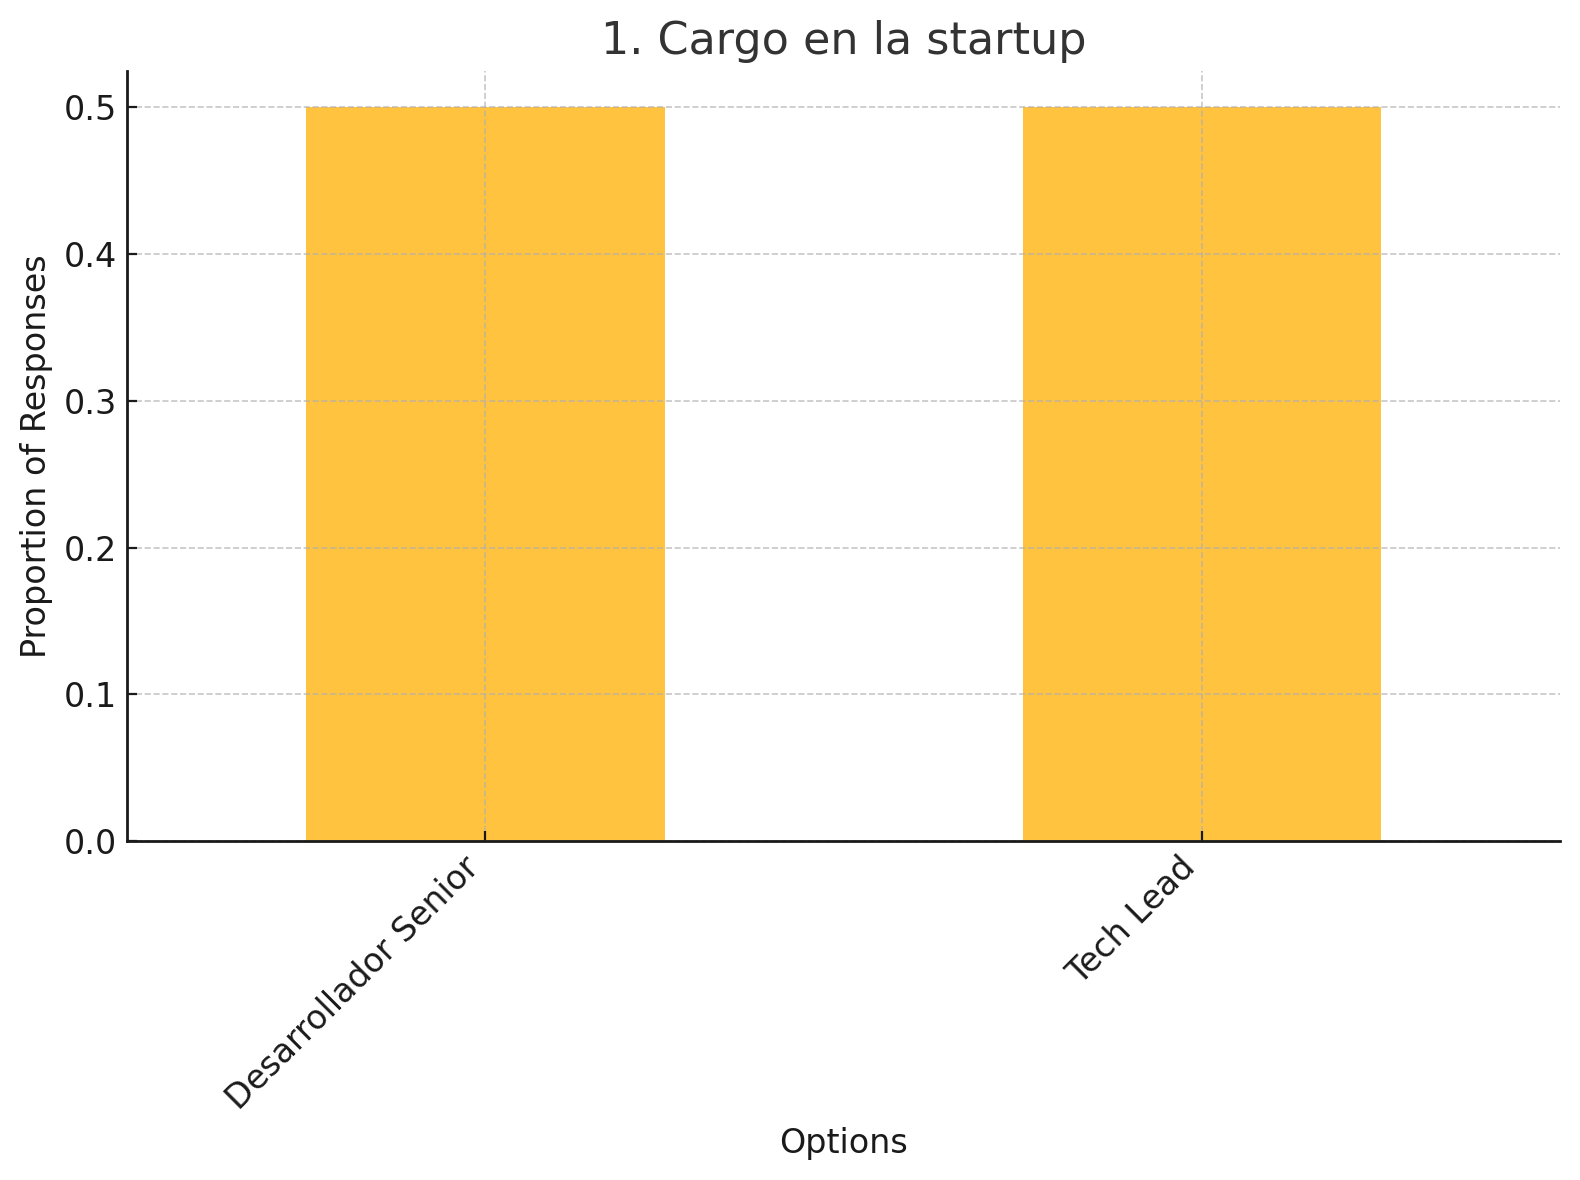
\includegraphics[width=8cm]{images/question1.png}
    \centering
\end{figure}

Conclusión: La mayoría de los encuestados ocupan cargos de Tech Lead o Desarrollador Senior de forma equilibrada, lo que indica que las respuestas reflejan tanto decisiones estratégicas como prácticas en el uso de tecnologías.\\

\textbf{2. ¿Cuántos años de experiencia tiene en el desarrollo de aplicaciones móviles?}

\begin{figure}[h!]
    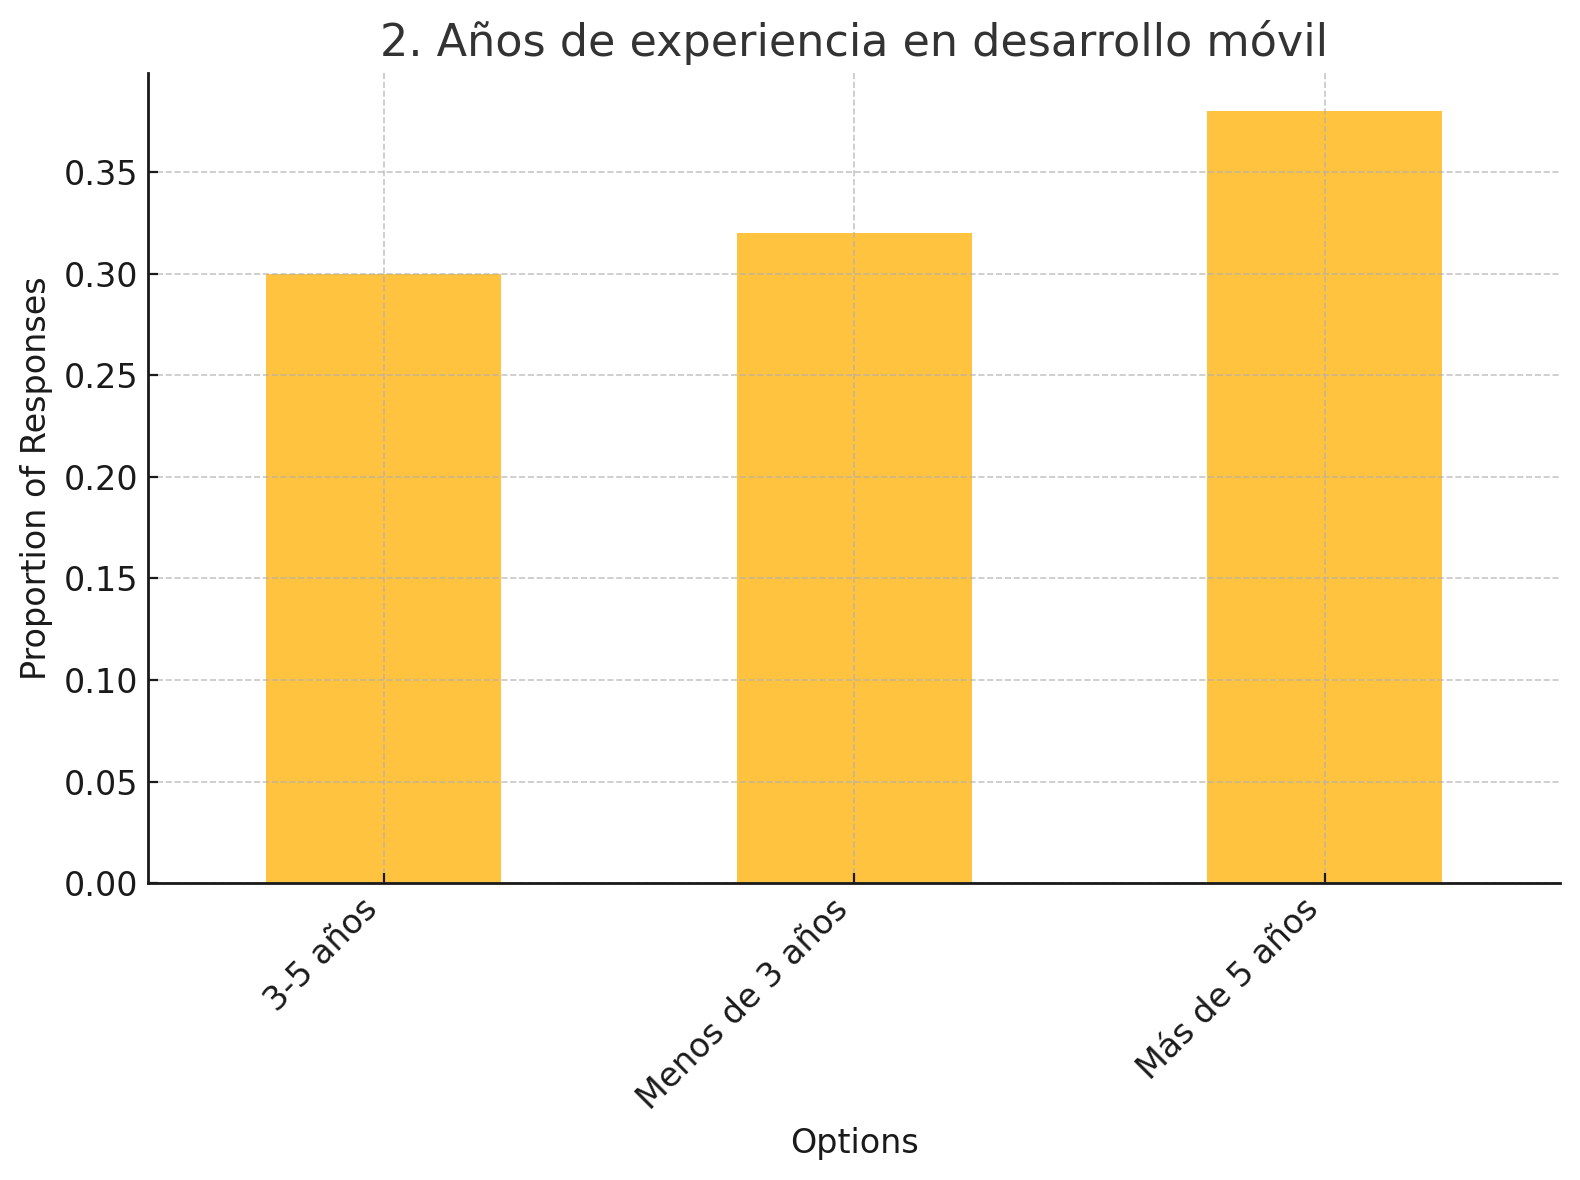
\includegraphics[width=8cm]{images/question2.png}
    \centering
\end{figure}

Conclusión: Predominan los participantes con más de 5 años de experiencia, sugiriendo una perspectiva más informada sobre las ventajas y desventajas de las tecnologías multiplataforma.\\

\textbf{3. ¿Qué tipo de tecnologías utiliza principalmente en su trabajo?}

\begin{figure}[h!]
    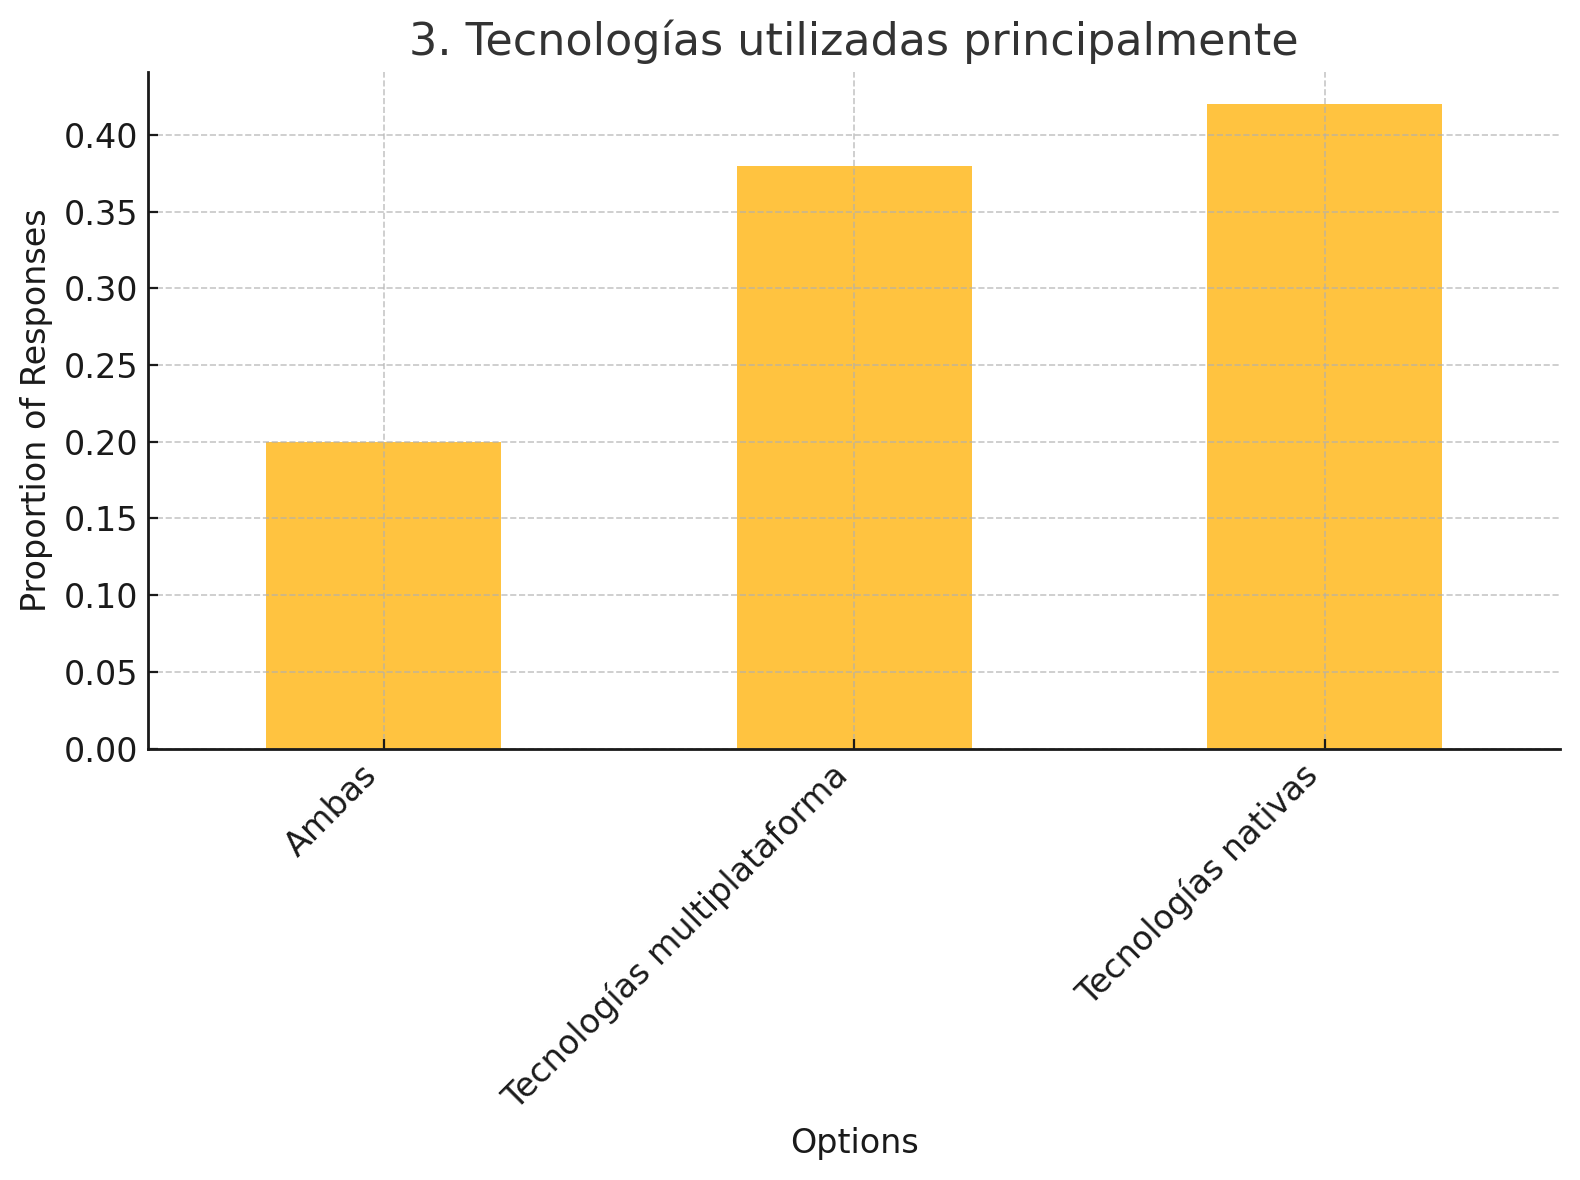
\includegraphics[width=8cm]{images/question3.png}
    \centering
\end{figure}

Conclusión: Un equilibrio entre nativas, multiplataforma y mixto muestra que las empresas adoptan diferentes estrategias dependiendo de sus necesidades específicas.\\

\textbf{4. ¿En qué medida considera que las tecnologías multiplataforma reducen los
costos de desarrollo en comparación con las tecnologías nativas?}

\begin{figure}[h!]
    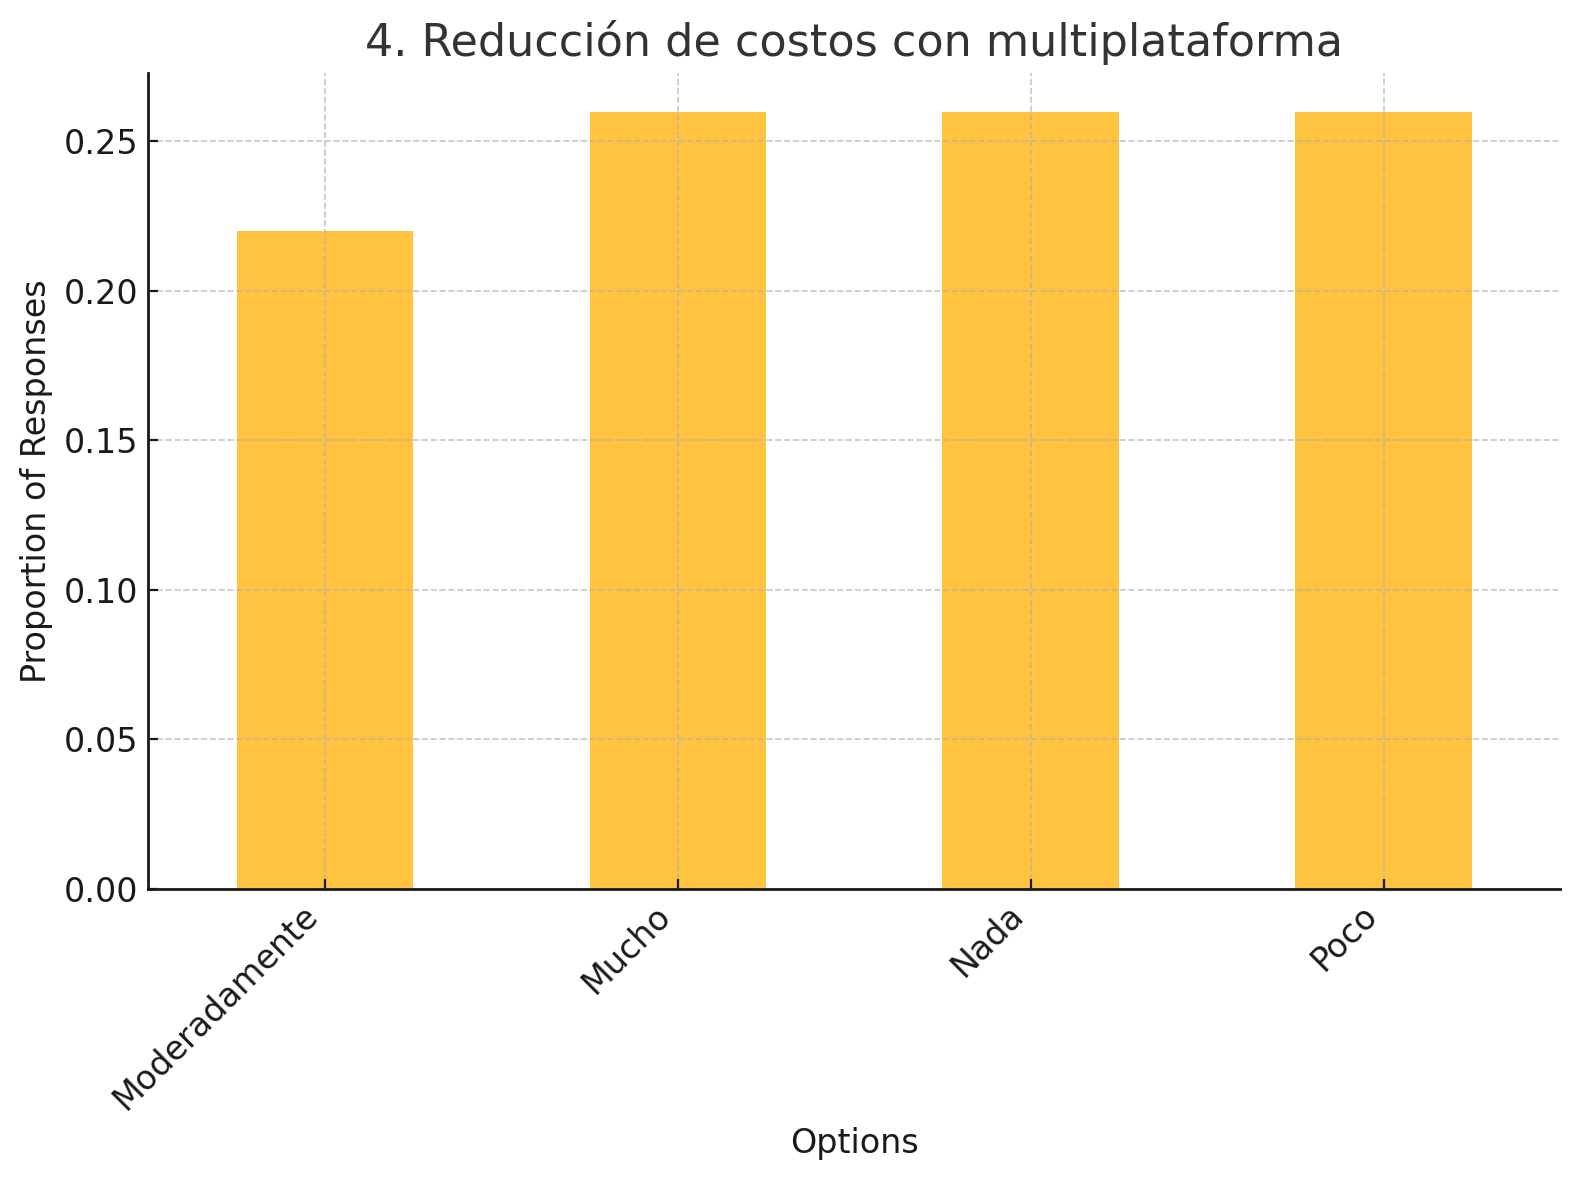
\includegraphics[width=8cm]{images/question4.png}
    \centering
\end{figure}

Conclusión: La mayoría considera que las tecnologías multiplataforma reducen costos moderadamente o mucho, indicando una percepción positiva en términos económicos.\\

\newpage
\textbf{5. Según su experiencia, ¿las tecnologías multiplataforma permiten acortar los
tiempos de desarrollo?}

\begin{figure}[h!]
    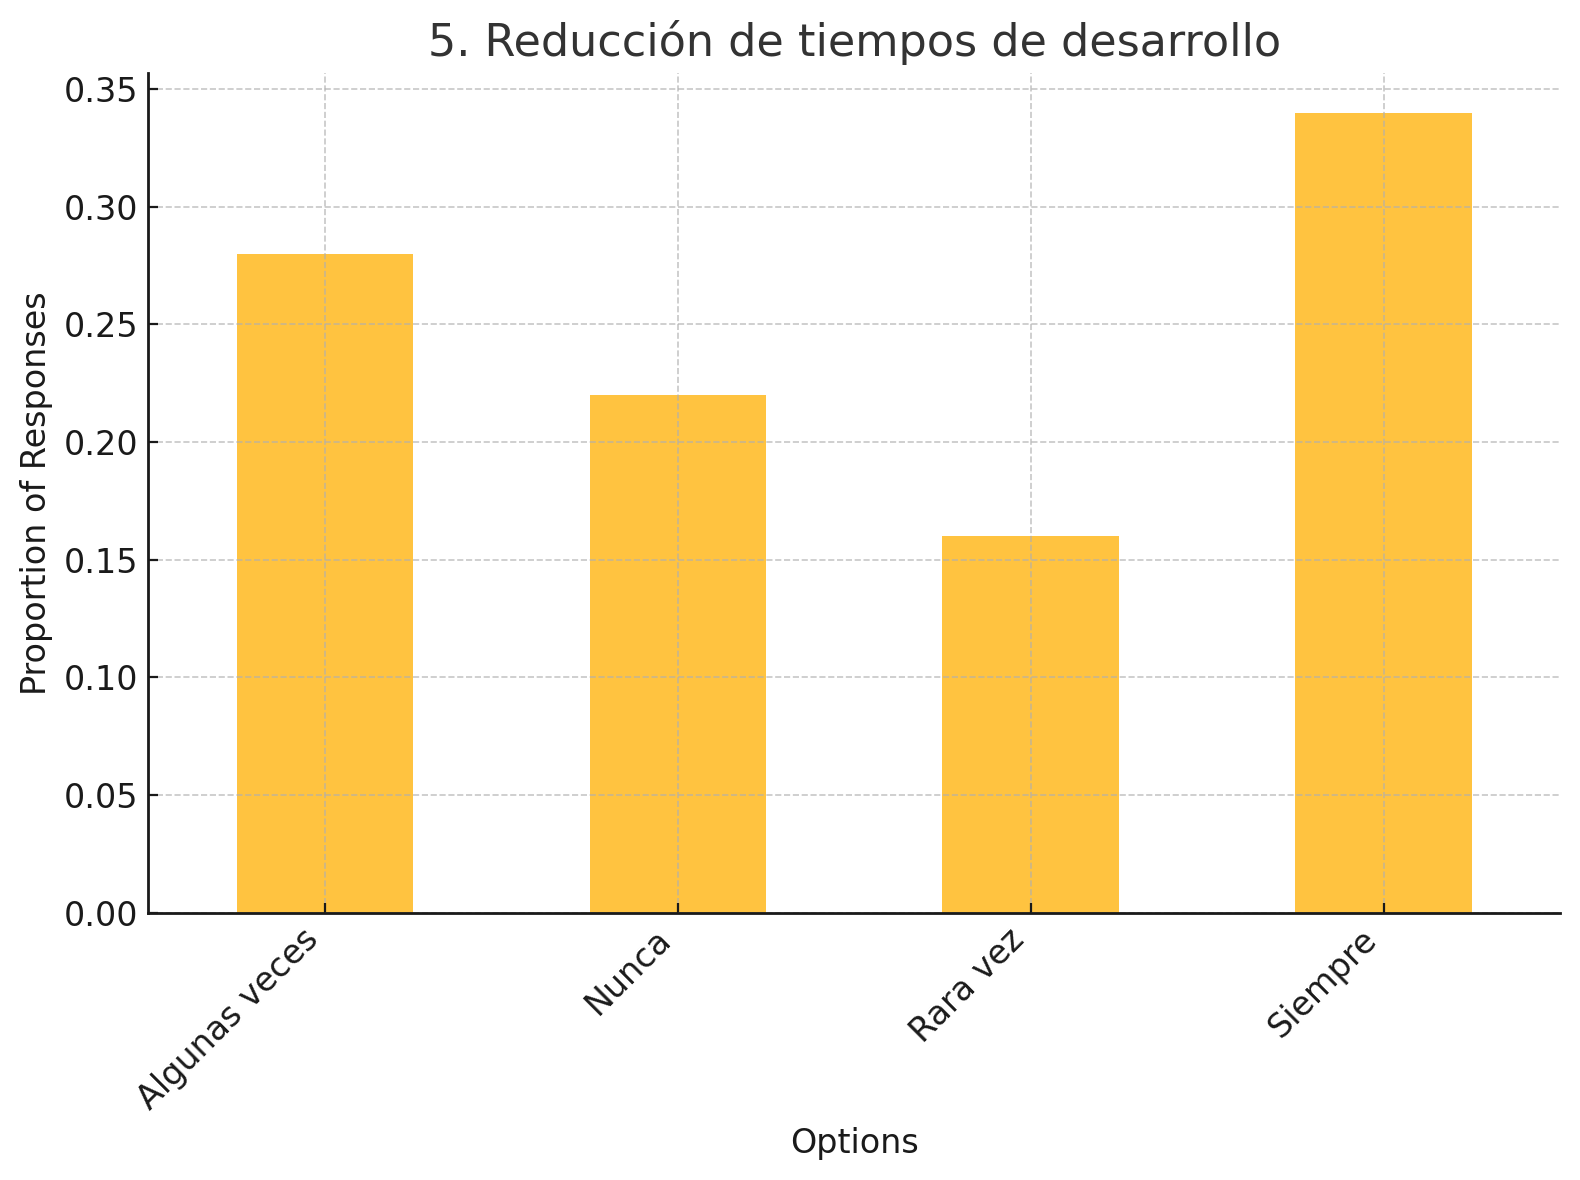
\includegraphics[width=8cm]{images/question5.png}
    \centering
\end{figure}

Conclusión: La percepción está dividida, aunque una buena proporción indica que “algunas veces” o “siempre” reducen tiempos, subrayando la eficiencia esperada de estas tecnologías.\\

\textbf{6. ¿Qué porcentaje del presupuesto de un proyecto, en promedio, se reduce
utilizando tecnologías multiplataforma?}

\begin{figure}[h!]
    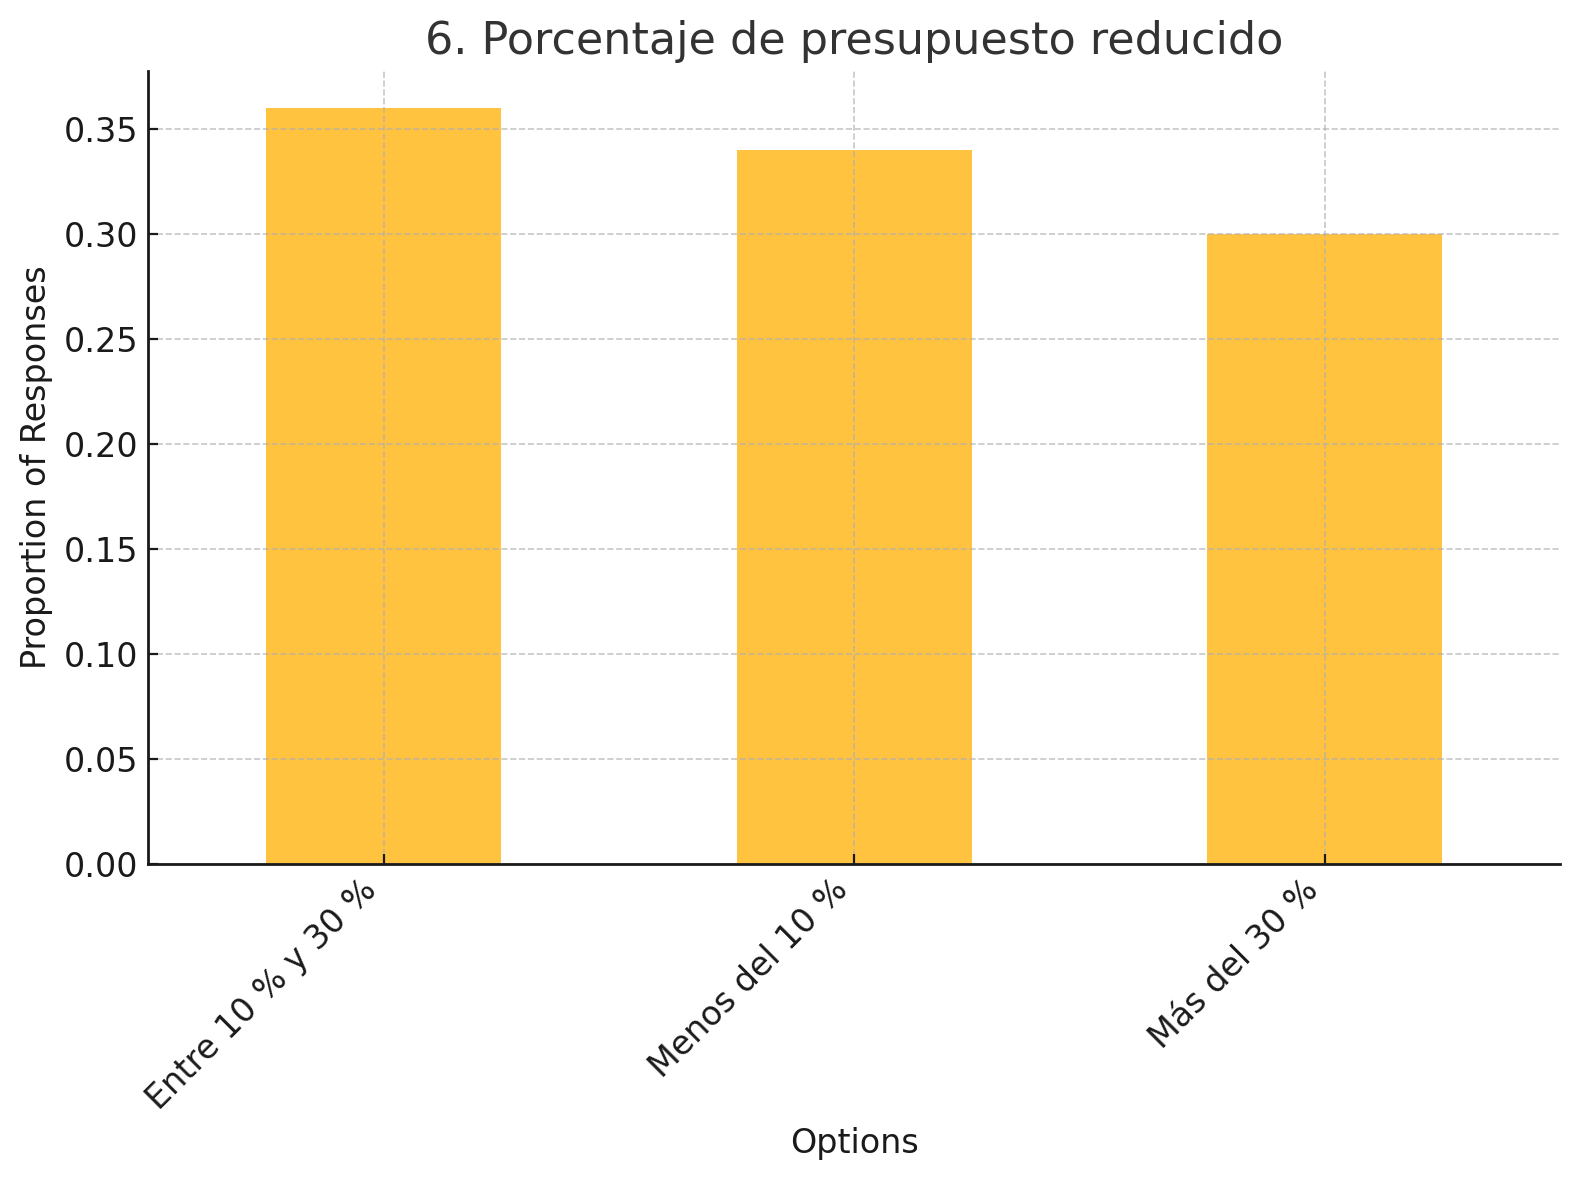
\includegraphics[width=8cm]{images/question6.png}
    \centering
\end{figure}

Conclusión: Más del 30 \% y 10-30 \% dominan, evidenciando un impacto notable en los presupuestos al usar tecnologías multiplataforma.\\

\newpage
\textbf{7. ¿Qué tan fácil es el mantenimiento de aplicaciones desarrolladas con tec-
nologías multiplataforma en comparación con las nativas?}

\begin{figure}[h!]
    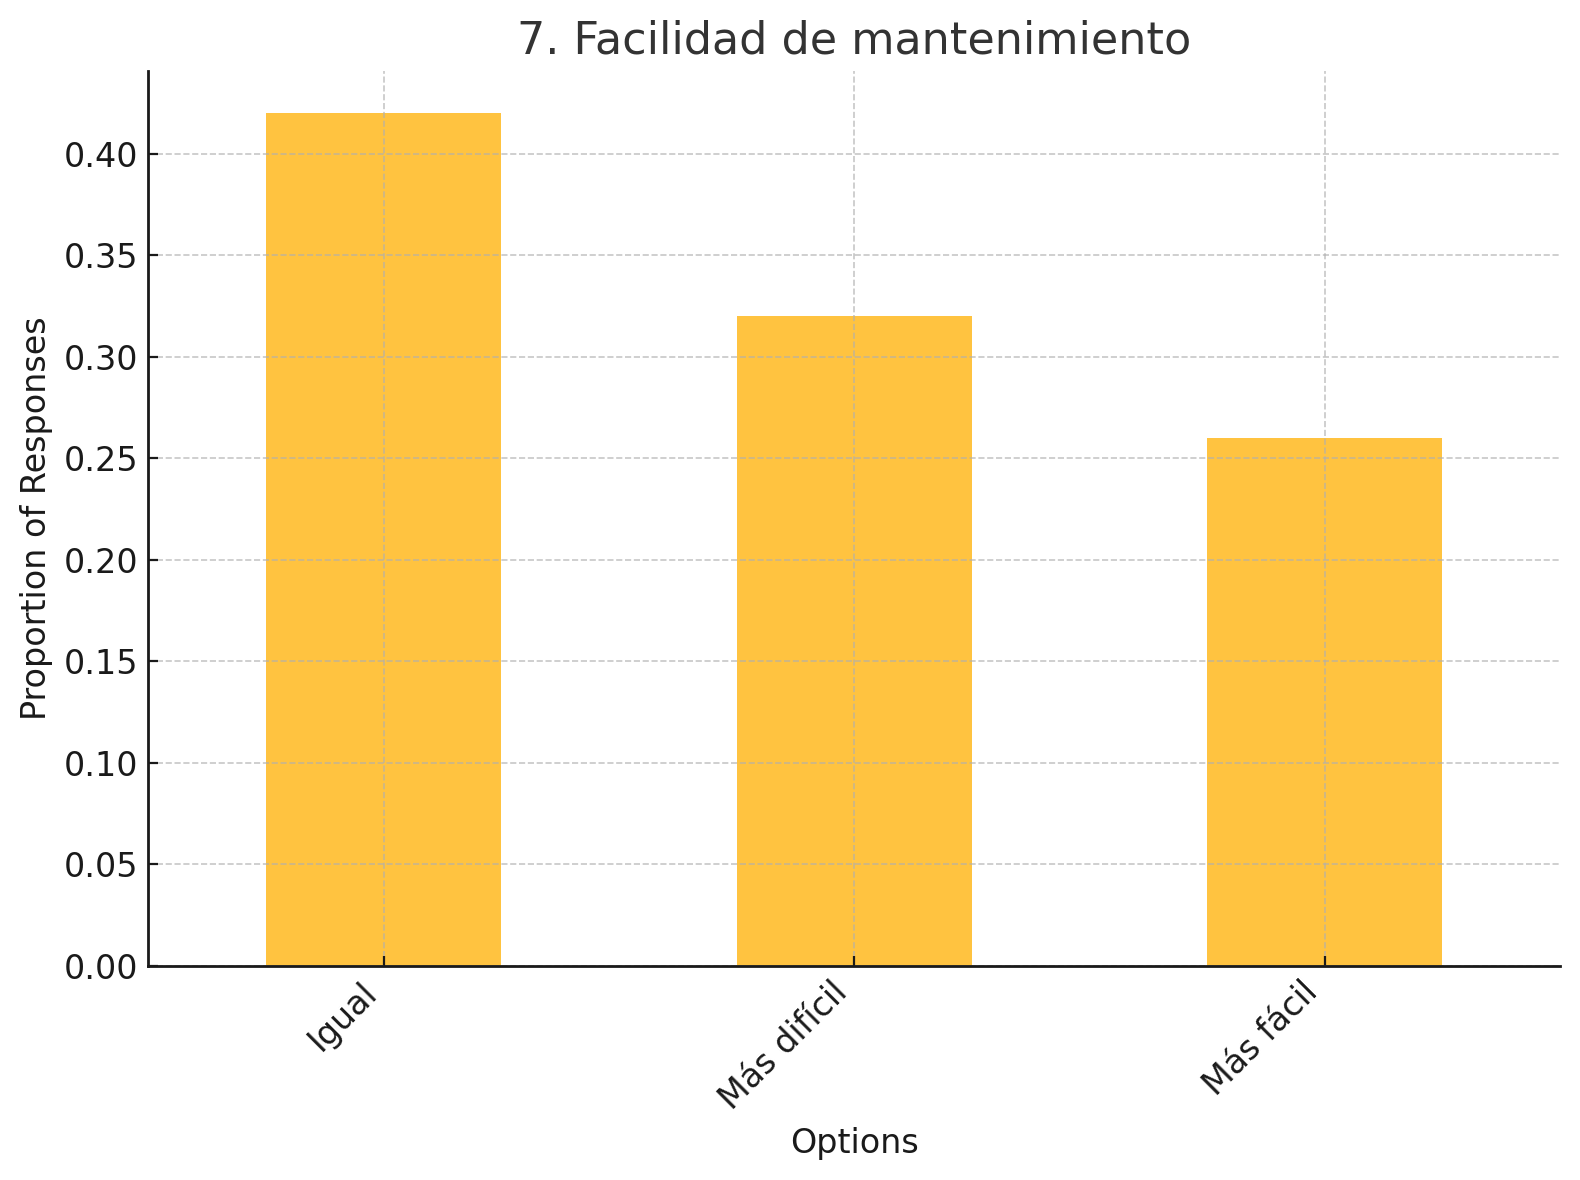
\includegraphics[width=8cm]{images/question7.png}
    \centering
\end{figure}

Conclusión: Predomina la percepción de que el mantenimiento es igual o más fácil con tecnologías multiplataforma, lo que refuerza su viabilidad en proyectos.\\

\textbf{8. En términos de calidad de la experiencia del usuario, ¿cómo califica el ren-
dimiento de las aplicaciones multiplataforma frente a las nativas?}

\begin{figure}[h!]
    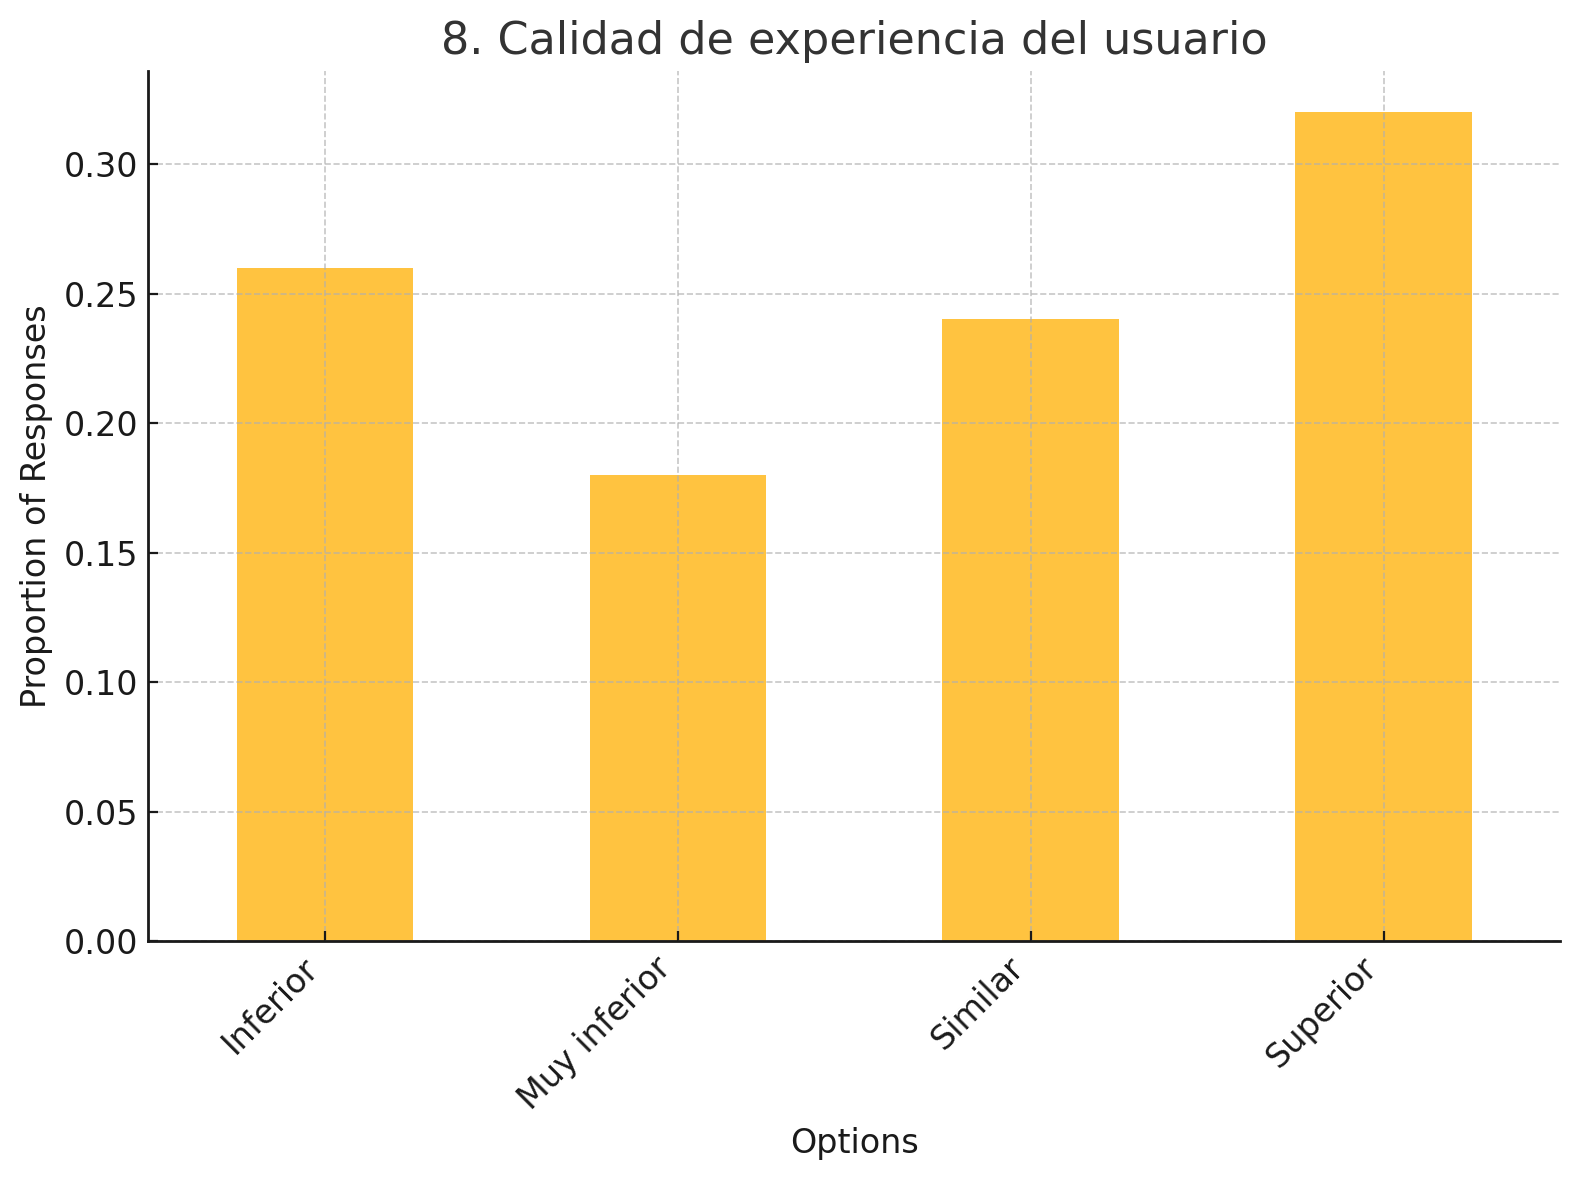
\includegraphics[width=8cm]{images/question8.png}
    \centering
\end{figure}

Conclusión: La calidad se percibe mayoritariamente como similar o superior, lo que indica que las limitaciones técnicas no afectan significativamente la experiencia del usuario.\\

\newpage
\textbf{9. ¿Qué tan frecuentemente enfrenta problemas de compatibilidad en proyec-
tos multiplataforma?}

\begin{figure}[h!]
    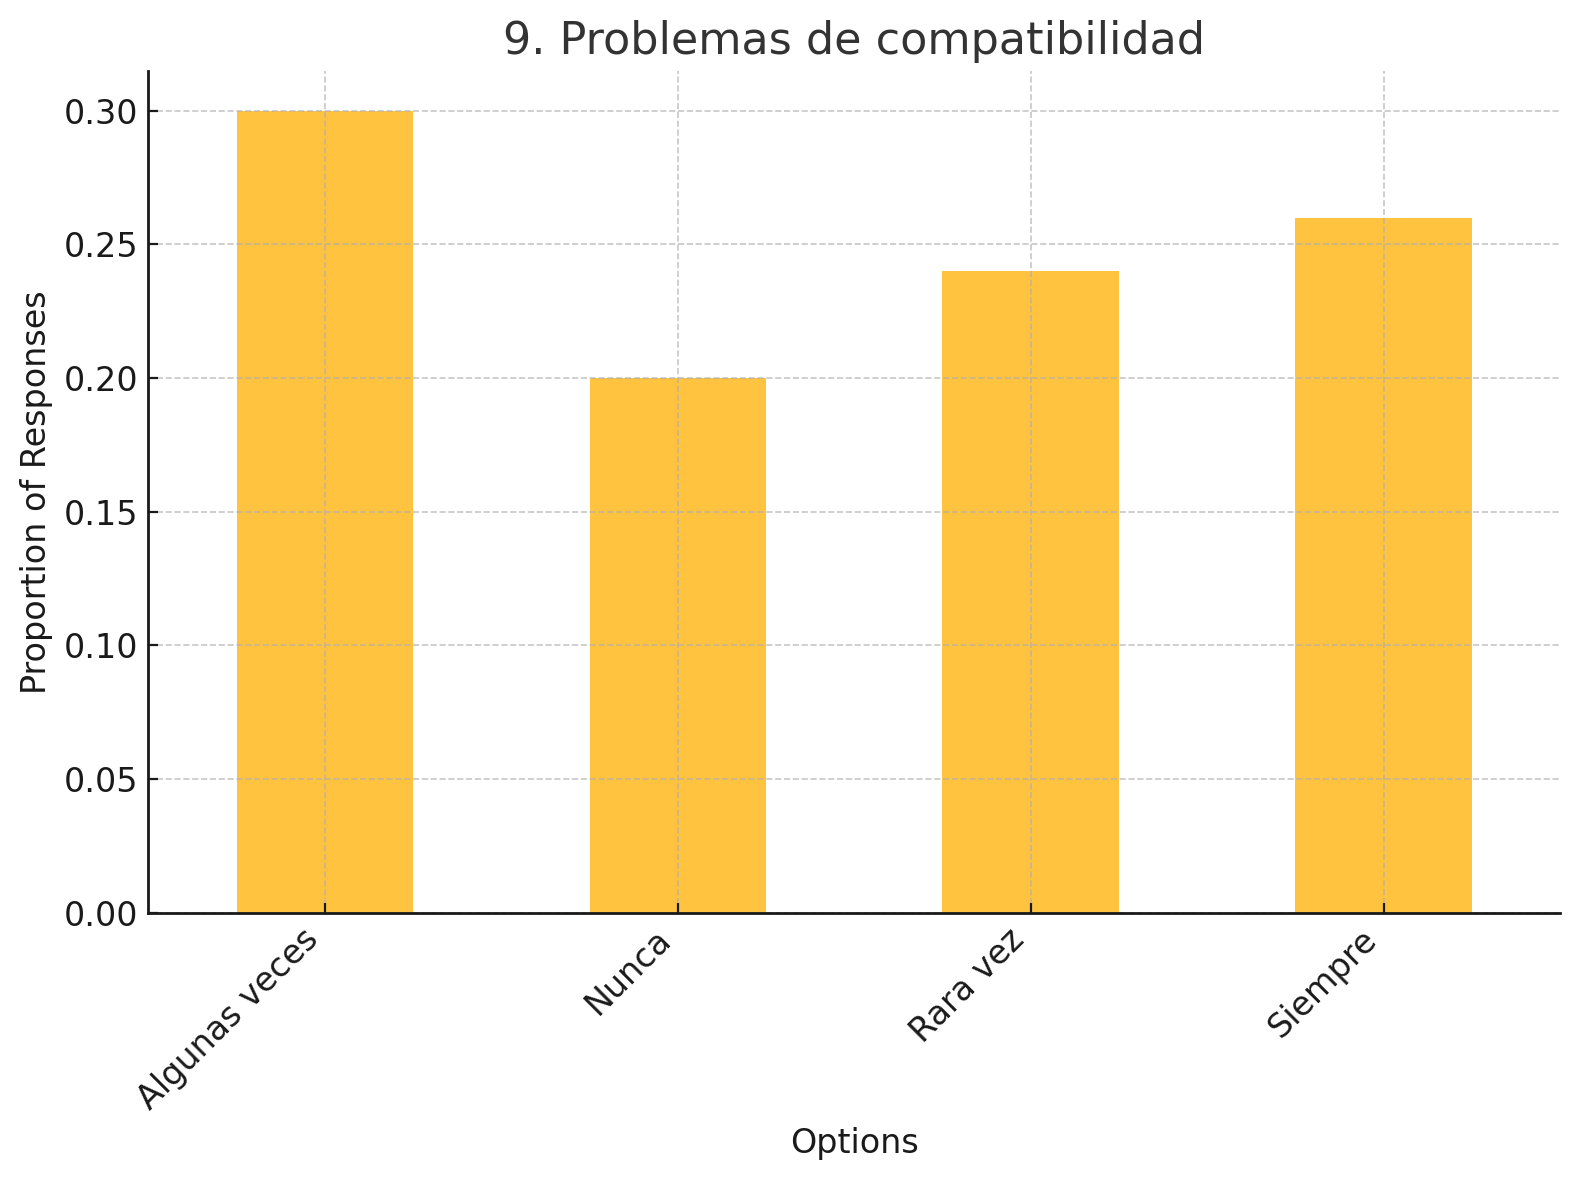
\includegraphics[width=8cm]{images/question9.png}
    \centering
\end{figure}

Conclusión: Aunque hay quienes enfrentan problemas algunas veces, la mayoría los experimenta rara vez o nunca, destacando mejoras en la compatibilidad.\\

\textbf{10. ¿Cuál es su nivel de satisfacción general con el uso de tecnologías multi-
plataforma en proyectos móviles?}

\begin{figure}[h!]
    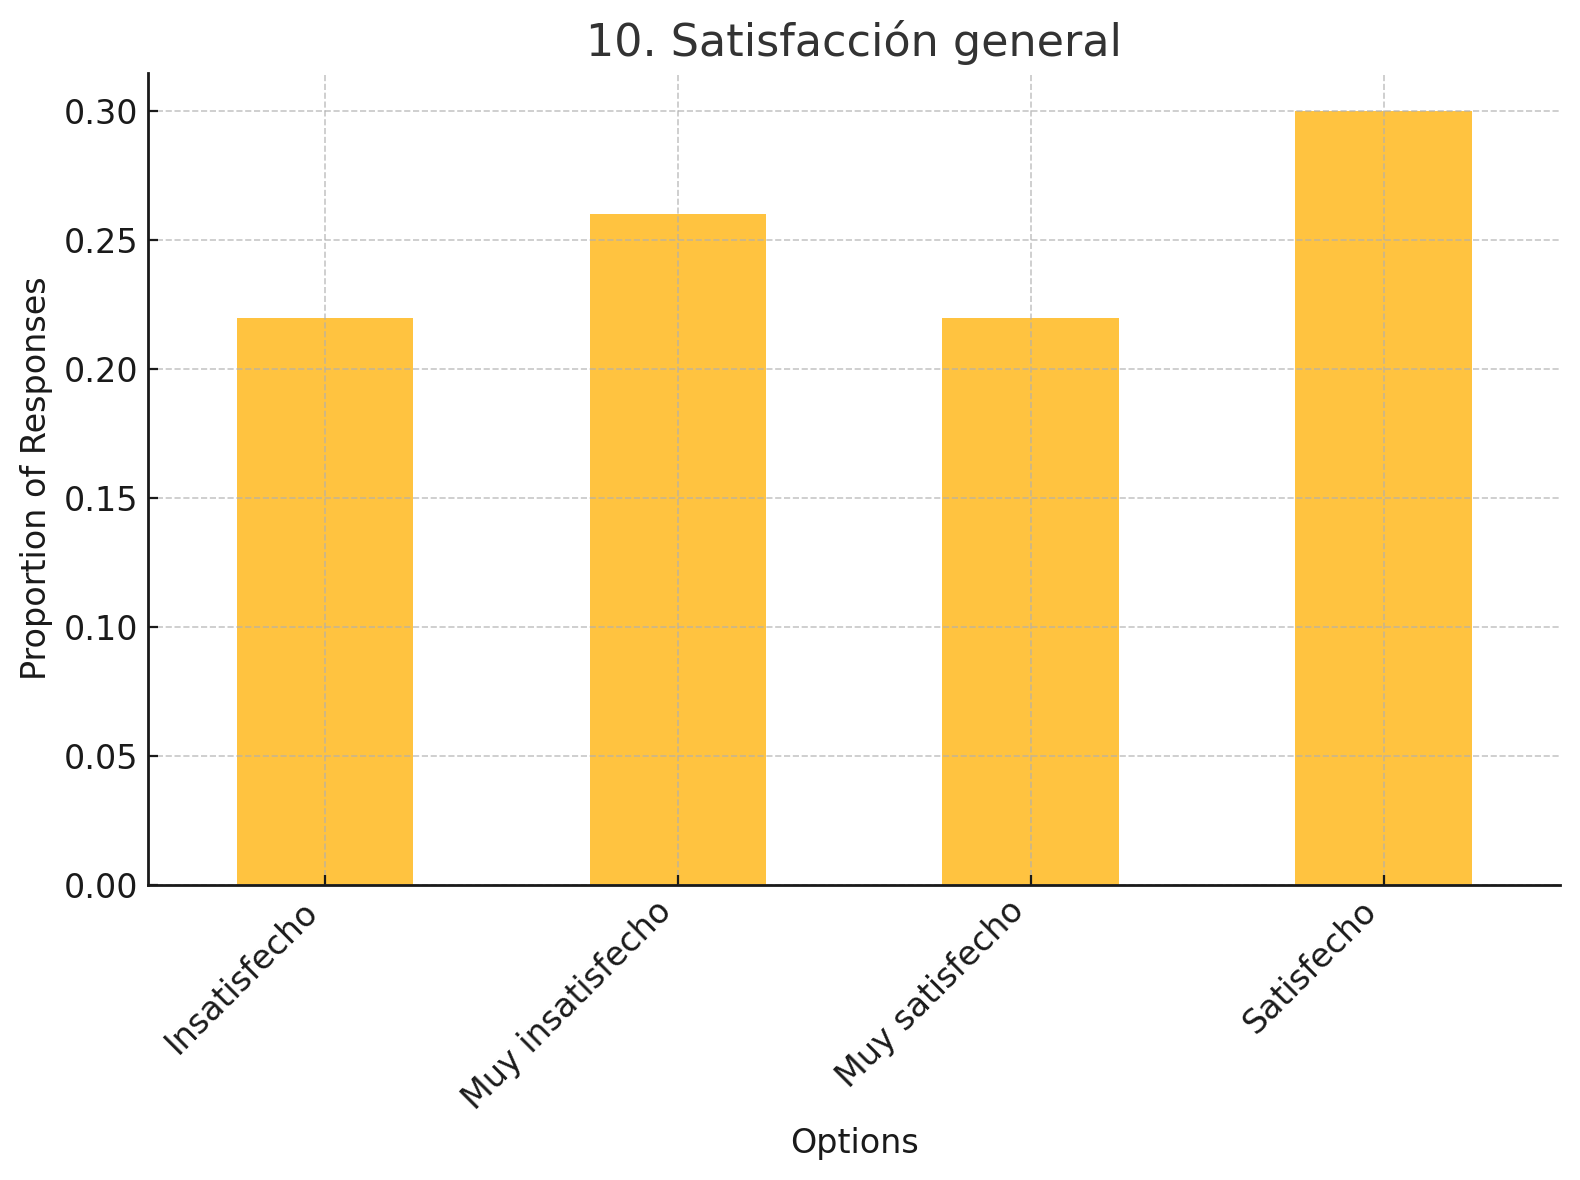
\includegraphics[width=8cm]{images/question10.png}
    \centering
\end{figure}

Conclusión: La satisfacción general es alta, con muchos encuestados indicando estar satisfechos o muy satisfechos, validando la confianza en tecnologías multiplataforma.\\

\newpage
\textbf{11. ¿Qué tan probable es que recomiende el uso de tecnologías multiplatafor-
ma para proyectos futuros?}

\begin{figure}[h!]
    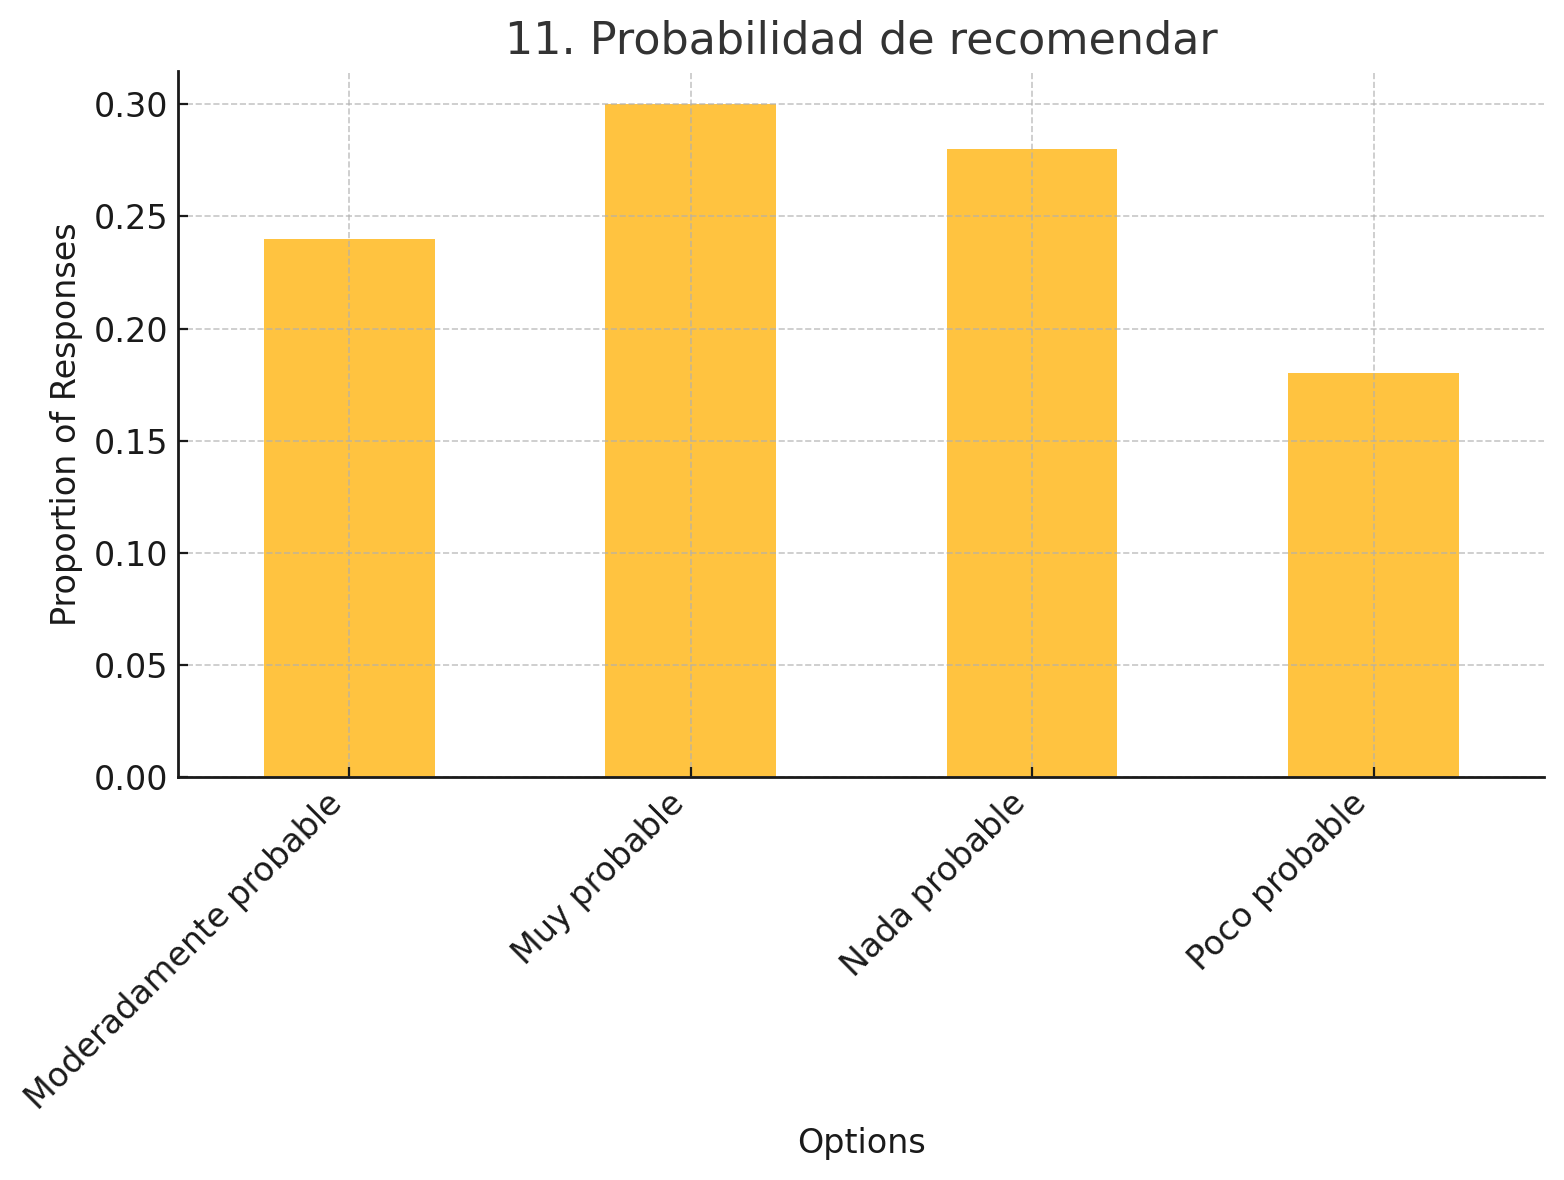
\includegraphics[width=8cm]{images/question11.png}
    \centering
\end{figure}

Conclusión: Las respuestas indican una alta probabilidad de recomendación, con muchos participantes considerando esta tecnología como moderadamente o muy probable de recomendar.\\

\textbf{12. ¿Considera que las tecnologías multiplataforma son una solución sosteni-
ble a largo plazo para el desarrollo de aplicaciones móviles?}

\begin{figure}[h!]
    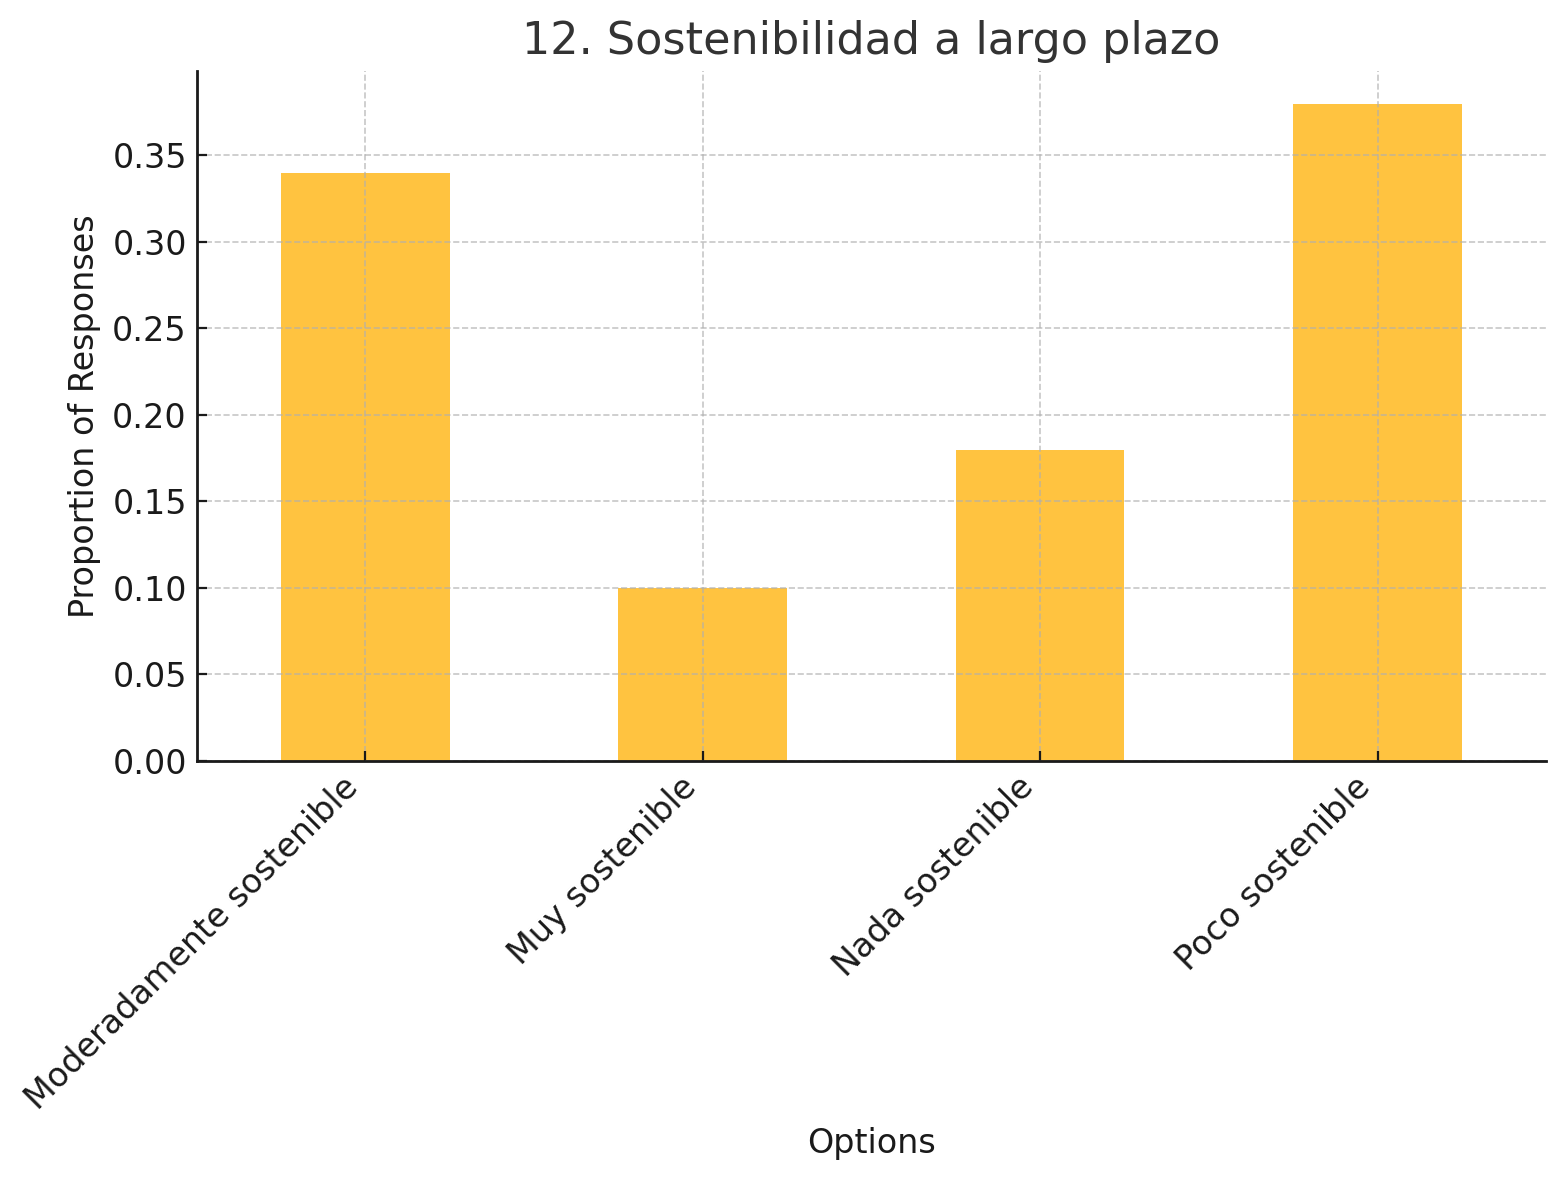
\includegraphics[width=8cm]{images/question12.png}
    \centering
\end{figure}

Conclusión: La mayoría considera que las tecnologías multiplataforma son moderadamente o muy sostenibles, destacando su potencial como solución a largo plazo.

\newpage
\subsection{Conclusiones generales}

La programación multiplataforma se caracteriza por su enfoque en reutilizar código para múltiples sistemas operativos, reduciendo redundancias. Frameworks como Flutter, React Native y Xamarin son ampliamente adoptados debido a su flexibilidad, soporte robusto y facilidad de integración, ofreciendo una alternativa viable a los entornos nativos.\\

El desarrollo multiplataforma tiende a reducir los costos al minimizar la duplicación de esfuerzos para múltiples plataformas. Sin embargo, los costos iniciales de aprendizaje, herramientas específicas y la necesidad de optimizaciones técnicas pueden influir en la relación costo-beneficio, especialmente en proyectos complejos.\\

Aunque las aplicaciones nativas ofrecen un rendimiento óptimo y acceso total a las capacidades del dispositivo, las multiplataforma han mejorado significativamente, ofreciendo una experiencia de usuario comparable y funcionalidad suficiente para la mayoría de los casos, salvo en aplicaciones que exigen máxima precisión o personalización.\\

El desarrollo multiplataforma permite ahorros sustanciales de tiempo y costos al compartir código entre plataformas, especialmente en proyectos con recursos limitados. Además, el mantenimiento es más eficiente al centralizar las actualizaciones en una base de código única, lo que lo hace una opción práctica para empresas pequeñas y medianas.\\

Se recomienda adoptar frameworks multiplataforma como Flutter o React Native para proyectos con requerimientos generales, priorizando evaluaciones iniciales de necesidades específicas. Las empresas con recursos limitados deben enfocarse en proyectos con menor complejidad nativa y aprovechar las comunidades y recursos gratuitos disponibles para formación y soporte.\\